% paper/sections/10b_component_verification.tex
%
% §10.3  コンポーネント検証結果（実施済み・仕様）
%   §10.3.1: CLS 保存性評価（動的非一様格子）← 10b_cls_conservation.tex
%   §10.3.2: CCD 仮想時間ソルバー精度検証    ← 10b_ccd_pseudotime_verification.tex
%   §10.3.3: CCD-Poisson ソルバー単体検証    ← 10b_ppe_verification.tex

\subsection{コンポーネント検証結果（実施済み）}
\label{sec:component_verification}

以下に，各サブシステムの単体検証実験を示す．
いずれも §\ref{sec:algorithm} の対応モジュールを独立に動かし，
表~\ref{tab:verification} の検証項目と直接対応する定量確認を行ったものである．

\subsubsection{CLS 保存性評価：動的非一様格子上での保存型再マッピング}
\label{app:cls_conservation}
\input{sections/10b_cls_conservation}

\subsubsection{仮想時間陰解法と CCD の精度検証}
\label{app:ccd_pseudotime}
% paper/sections/10b_ccd_pseudotime_verification.tex
%
% §10.3.2  仮想時間陰解法 + CCD の精度検証（3事例）
%          （旧 D.8; \section と \label は 10b_component_verification.tex の
%            \subsubsection で提供する）
%      Case 1: Poisson（空間収束），Case 2: 拡散方程式（大 Δt 安定性），
%      Case 3: 定常移流拡散（高 Pe 境界層）
%
% 実験スクリプト: experiments/ccd_pseudotime_verification.py
% 結果データ:    results/ccd_pseudotime/

% ═══════════════════════════════════════════════════════════════════════════════

本節は，6次精度 CCD スキーム（§\ref{sec:CCD}）と
仮想時間陰解法（§\ref{sec:ppe_pseudotime}）の組み合わせが，
標準 2次中心差分（CDS2）と比較してどの程度の精度優位をもたらすかを
3種類の標準問題によって定量的に検証した記録である．

% ─────────────────────────────────────────────────────────────────────────────
\paragraph{Case 1：空間収束性（\texorpdfstring{$u'' = -(2\pi)^2\sin(2\pi x)$}{u'' = -(2pi)\^{}2 sin(2pi x)}）}\label{app:ccd_case1}
% ─────────────────────────────────────────────────────────────────────────────

\paragraph{設定}
$u(x) = \sin(2\pi x)$，$x \in [0,1]$ の 2 階微分を CCD および CDS2 で計算し，
格子サイズ $N \in \{8, 16, 32, 64, 128\}$（節点数 $N+1$，格子間隔 $h=1/N$）に対する
$L^\infty$ 誤差の収束次数を測定する．

\paragraph{結果}
表~\ref{tab:ccd_case1} に誤差と収束次数を示す．

\begin{table}[htbp]
  \centering
  \caption{%
    $u'' = -(2\pi)^2\sin(2\pi x)$ の $L^\infty$ 誤差（内部節点 $i = 1 \ldots N-1$）．
    CCD の収束次数は境界スキームの精度（Eq-I-bc: $O(h^5)$，Eq-II-bc: $O(h^4)$）に
    制限され，漸近的に $O(h^5)$ に収束する（内部ステンシルの $O(h^6)$ は
    近傍節点を通じて境界誤差の影響を受ける）．
  }
  \label{tab:ccd_case1}
  \begin{tabular}{rcccc}
    \toprule
    $N$ & CCD $L^\infty$ & CDS2 $L^\infty$ & CCD order & CDS2 order \\
    \midrule
      8 & $9.73 \times 10^{-1}$ & $1.99 \times 10^{0}$  & --   & --   \\
     16 & $5.03 \times 10^{-2}$ & $5.05 \times 10^{-1}$ & 4.28 & 1.98 \\
     32 & $1.76 \times 10^{-3}$ & $1.27 \times 10^{-1}$ & 4.83 & 1.99 \\
     64 & $5.67 \times 10^{-5}$ & $3.17 \times 10^{-2}$ & 4.96 & 2.00 \\
    128 & $1.78 \times 10^{-6}$ & $7.93 \times 10^{-3}$ & 4.99 & 2.00 \\
    \bottomrule
  \end{tabular}
\end{table}

\begin{figure}[htbp]
  \centering
  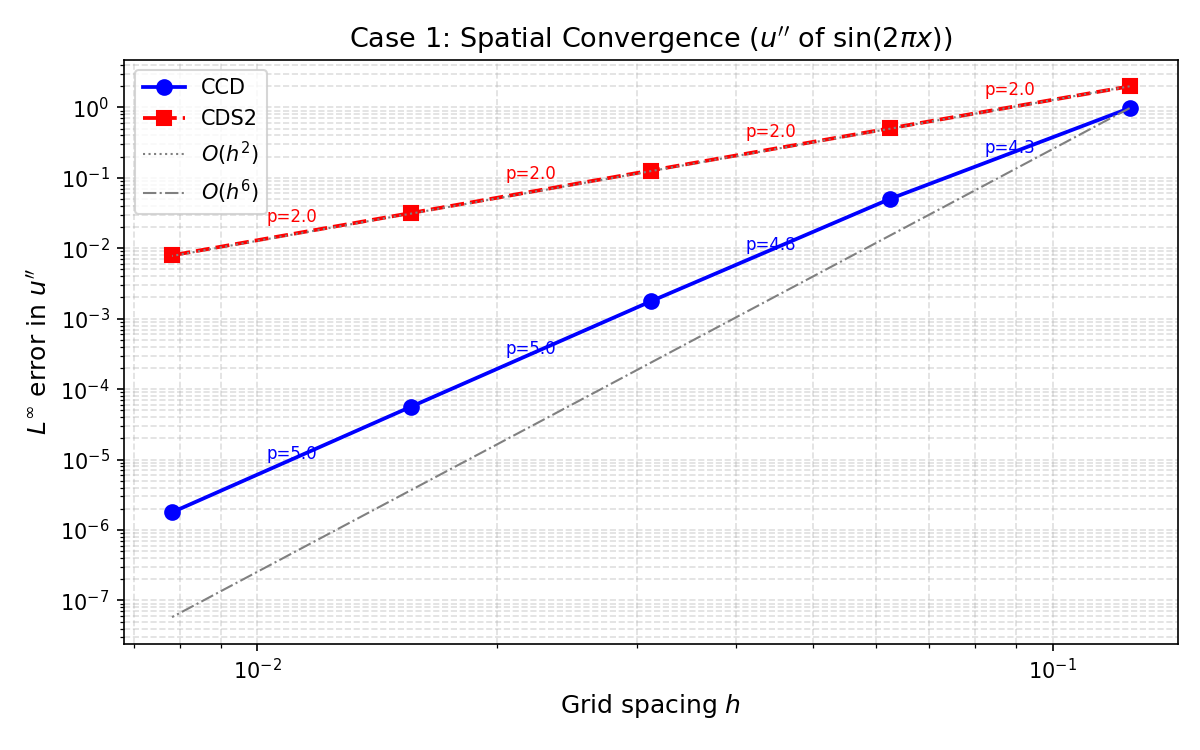
\includegraphics[width=0.72\linewidth]{figures/case1_convergence.png}
  \caption{%
    Case 1：格子間隔 $h$ に対する $L^\infty$ 誤差の収束グラフ（両対数）．
    CCD は漸近的に $O(h^5)$（破線：$O(h^6)$ 参照線），
    CDS2 は $O(h^2)$ で収束する．
  }
  \label{fig:ccd_case1}
\end{figure}

\begin{tcolorbox}[resultbox, title={空間収束次数（CCD vs.\ CDS2）}]
  \begin{itemize}
    \item CCD は内部ステンシル $O(h^6)$ を持つが，コンパクトスキームの結合を通じた
          境界スキーム $O(h^5)$（Eq-I-bc）の影響により，
          全域 $L^\infty$ 収束次数は $O(h^5)$ に制限される（$N=128$ で $p \approx 5.0$）．
    \item $N=128$ の時点で CCD の誤差は CDS2 の約 4500 倍小さい
          （$1.78 \times 10^{-6}$ vs.\ $7.93 \times 10^{-3}$）．
    \item CDS2 は厳密に $O(h^2)$ で収束し，格子収束挙動は単純かつ予測可能である．
  \end{itemize}
\end{tcolorbox}

% ─────────────────────────────────────────────────────────────────────────────
\paragraph{Case 2：拡散方程式における大 \texorpdfstring{$\Delta t$}{Δt} 安定性．}\label{app:ccd_case2}
% ─────────────────────────────────────────────────────────────────────────────

\paragraph{設定}
\begin{equation}
  \frac{\partial u}{\partial t} = \varepsilon\,\frac{\partial^2 u}{\partial x^2},
  \qquad x \in [0,1],\quad u(0,t)=u(1,t)=0,\quad u(x,0)=\sin(\pi x),
  \label{eq:ccd_parabolic}
\end{equation}
$\varepsilon = 0.01$，$T = 1$ の厳密解 $u(x,T) = e^{-\varepsilon\pi^2 T}\sin(\pi x)$
を用いて $N = 64$（$h = 1/64$）で検証する．

\paragraph{時間積分法}
物理時間は BDF2 で前進させ，各ステップで生じる Helmholtz 型連立方程式
\begin{equation}
  \frac{3}{2\Delta t}\,u^{n+1} - \varepsilon\,\frac{\partial^2 u^{n+1}}{\partial x^2}
  = \frac{4u^n - u^{n-1}}{2\Delta t}
  \label{eq:ccd_helmholtz}
\end{equation}
を仮想時間前進 Euler 法で反復求解する：
\begin{equation}
  u^{m+1} = u^m + \Delta\tau\!\left(
    f - \frac{3}{2\Delta t}\,u^m + \varepsilon\,\partial^2_x u^m
  \right),
  \label{eq:ccd_pseudotime}
\end{equation}
ただし収束判定は $\|\text{残差}\|_\infty < 10^{-10}$，
最大反復回数 500 回とする．

\paragraph{仮想時間刻み $\Delta\tau$ の設定}
仮想時間前進 Euler の安定条件は
\begin{equation}
  \Delta\tau \cdot \left(\frac{3}{2\Delta t} + \varepsilon\,\rho(D_2)\right) \leq 2
  \label{eq:ccd_dtau_stability}
\end{equation}
ただし $\rho(D_2)$ は空間差分作用素 $D_2$ のスペクトル半径（$L^2$ 最大固有値絶対値）．
本実験では $D_2$ 行列を直接構築して数値的に計算した結果，
\begin{equation}
  \rho_{\text{CCD}} \approx \frac{9.57}{h^2},
  \qquad
  \rho_{\text{CDS2}} = \frac{4.0}{h^2}
  \label{eq:ccd_spectral_radius}
\end{equation}
となり，CCD の $D_2$ スペクトル半径は CDS2 の約 2.4 倍大きい．
式~\eqref{eq:ccd_dtau_stability} を満たすよう，各スキームに対して
\begin{equation}
  \Delta\tau = \frac{0.9}{\dfrac{3}{2\Delta t} + \dfrac{\varepsilon\,\rho(D_2)}{2}}
  \label{eq:ccd_dtau}
\end{equation}
を設定した（安定余裕を 10\% 確保）．

\paragraph{結果}
表~\ref{tab:ccd_case2} に $\Delta t_{\mathrm{phys}} \in \{\Delta t_{\mathrm{CFL}},\,0.01,\,0.1\}$
の 3 条件での $T=1$ における $L^\infty$ 誤差と 1 物理ステップあたりの
平均仮想時間反復回数を示す（$N=64$）．

\begin{table}[htbp]
  \centering
  \caption{%
    Case 2：拡散方程式 BDF2 + 仮想時間反復の精度比較（$N=64$，$\varepsilon=0.01$）．
    $\Delta t_{\mathrm{CFL}} = h^2/(2\varepsilon) \approx 0.0122$．
    太字：各 $\Delta t$ での最良値．
  }
  \label{tab:ccd_case2}
  \begin{tabular}{lcccc}
    \toprule
    $\Delta t_{\mathrm{phys}}$ & \multicolumn{2}{c}{$L^\infty$ 誤差 at $T=1$}
      & \multicolumn{2}{c}{平均反復回数 / ステップ} \\
    \cmidrule(lr){2-3}\cmidrule(lr){4-5}
     & CCD & CDS2 & CCD & CDS2 \\
    \midrule
    $\Delta t_{\mathrm{CFL}} \approx 0.0122$
      & $\mathbf{9.42 \times 10^{-7}}$ & $1.89 \times 10^{-5}$ & 51  & 29 \\
    $0.01$
      & $\mathbf{6.33 \times 10^{-7}}$ & $1.86 \times 10^{-5}$ & 44  & 26 \\
    $0.1$
      & $\mathbf{6.37 \times 10^{-5}}$ & $8.16 \times 10^{-5}$ & 318 & 141 \\
    \bottomrule
  \end{tabular}
\end{table}

\begin{figure}[htbp]
  \centering
  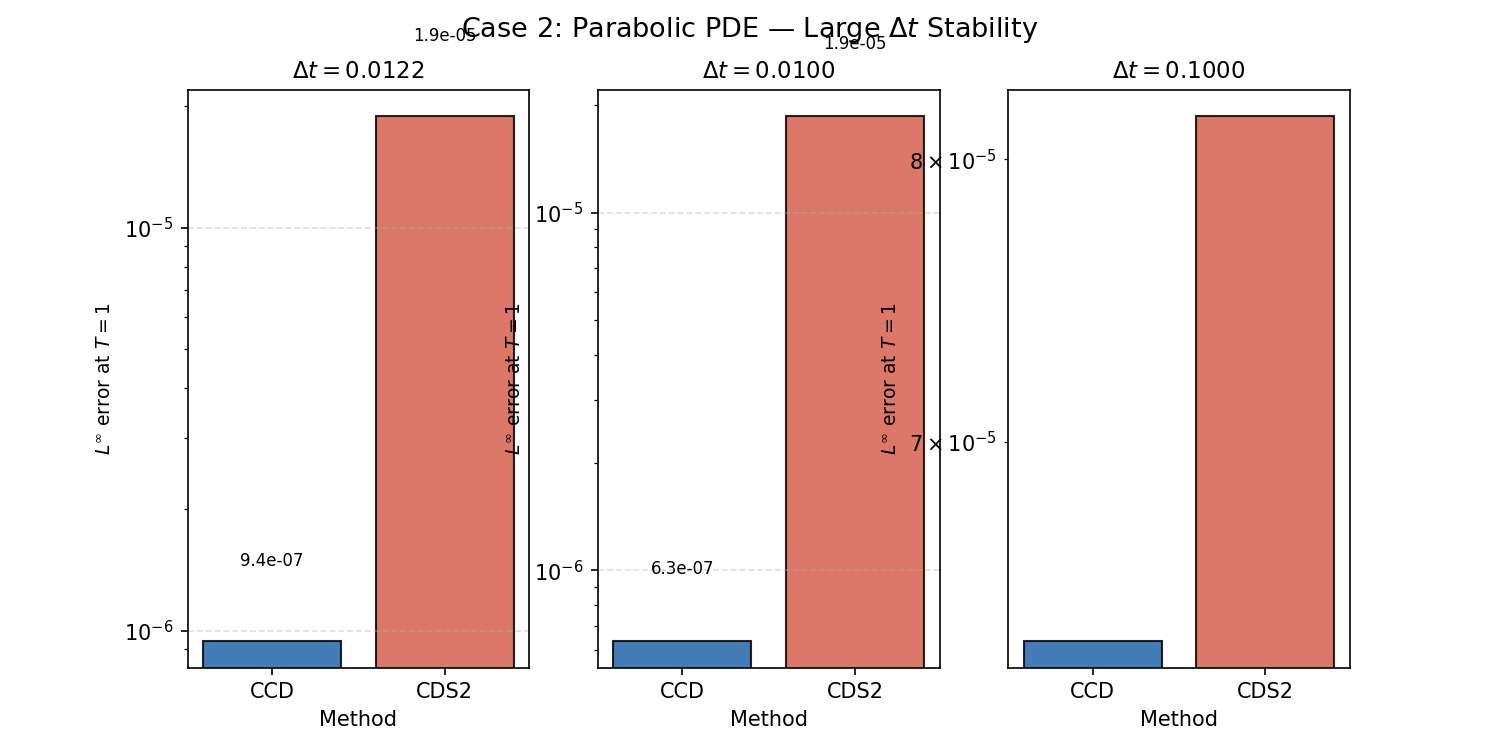
\includegraphics[width=0.88\linewidth]{figures/case2_parabolic.png}
  \caption{%
    Case 2：3 種の物理時間刻みにおける $T=1$ での $L^\infty$ 誤差の比較（棒グラフ）．
    小 $\Delta t$（空間誤差支配）では CCD が CDS2 より 20--30 倍精度が高い．
    大 $\Delta t = 0.1$（時間誤差支配）では両者の差が縮小する．
  }
  \label{fig:ccd_case2}
\end{figure}

\begin{tcolorbox}[resultbox, title={仮想時間陰解法における CCD の有効性}]
  \begin{itemize}
    \item 空間誤差が支配する小 $\Delta t$ 条件下では，CCD は CDS2 に比べ
          $L^\infty$ 誤差を約 20--30 倍低減する
          （$\Delta t = 0.01$：$6.33 \times 10^{-7}$ vs.\ $1.86 \times 10^{-5}$）．
    \item CCD の $D_2$ スペクトル半径は $\rho_{\text{CCD}} \approx 9.57/h^2$（CDS2 の 2.4 倍）
          であるため，安定な仮想時間刻みは CDS2 の約 1/2.4 となり，
          1 物理ステップあたりの反復回数も同比で増加する（51 vs.\ 29 回）．
    \item 大 $\Delta t = 0.1$ では時間誤差が支配的となり，CCD と CDS2 の誤差差は
          $1.3$ 倍程度に収束する．この条件では CCD 採用のメリットは限定的である．
  \end{itemize}
\end{tcolorbox}

% ─────────────────────────────────────────────────────────────────────────────
\paragraph{Case 3：定常移流拡散方程式（高 Péclet 境界層）．}\label{app:ccd_case3}
% ─────────────────────────────────────────────────────────────────────────────

\paragraph{設定}
\begin{equation}
  c\,\frac{\partial u}{\partial x} - \varepsilon\,\frac{\partial^2 u}{\partial x^2} = 0,
  \qquad x \in [0,1],\quad u(0)=0,\quad u(1)=1,
  \label{eq:ccd_advdiff}
\end{equation}
$c=1$，$\varepsilon = 0.1$（Péclet 数 $Pe = c/\varepsilon = 10$）の厳密解は
$u_{\rm exact}(x) = (e^{Pe\,x} - 1)/(e^{Pe} - 1)$．
格子サイズ $N \in \{8, 16, 32, 64, 128, 256\}$ に対して直接連立方程式で解く．

\paragraph{離散化}
CCD 作用素行列 $D_1$，$D_2$ を用いた線形系
\begin{equation}
  (c\,D_1 - \varepsilon\,D_2)\,\mathbf{u} = \mathbf{0},
  \qquad u_0 = 0,\quad u_N = 1,
  \label{eq:ccd_advdiff_sys}
\end{equation}
を scipy の直接 LU 分解で求解する．
CDS2 は標準中心差分 3 点ステンシルで同サイズの三重対角系を構築する．

\paragraph{結果}
表~\ref{tab:ccd_case3} に $L^\infty$ 誤差と収束次数を示す．
$Pe \cdot h = 2$（$N=5$，$h=0.2$）を超える粗格子では中心差分が
不安定を起こしうるが，本問題は定常方程式のため直接求解が可能であり，
$N=8$（$Pe \cdot h = 1.25$）から安定な結果が得られた．

\begin{table}[htbp]
  \centering
  \caption{%
    Case 3：定常移流拡散 $Pe=10$ の $L^\infty$ 誤差（内部節点）．
    太字：各 $N$ での最良値．
    $Pe \cdot h = 2$ の安定限界（$N=5$，$h=0.2$）はすでに $N=8$ で下回っている．
  }
  \label{tab:ccd_case3}
  \begin{tabular}{rccccc}
    \toprule
    $N$ & $Pe \cdot h$ & CCD $L^\infty$ & CDS2 $L^\infty$ & CCD order & CDS2 order \\
    \midrule
      8 & 1.250 & $\mathbf{6.77 \times 10^{-3}}$ & $5.57 \times 10^{-2}$ & --   & --   \\
     16 & 0.625 & $\mathbf{6.68 \times 10^{-4}}$ & $1.21 \times 10^{-2}$ & 3.34 & 2.20 \\
     32 & 0.312 & $\mathbf{2.85 \times 10^{-5}}$ & $3.02 \times 10^{-3}$ & 4.55 & 2.01 \\
     64 & 0.156 & $\mathbf{7.48 \times 10^{-7}}$ & $7.48 \times 10^{-4}$ & 5.25 & 2.01 \\
    128 & 0.078 & $\mathbf{1.52 \times 10^{-8}}$ & $1.87 \times 10^{-4}$ & 5.62 & 2.00 \\
    256 & 0.039 & $\mathbf{2.71 \times 10^{-10}}$ & $4.68 \times 10^{-5}$ & 5.81 & 2.00 \\
    \bottomrule
  \end{tabular}
\end{table}

\begin{figure}[htbp]
  \centering
  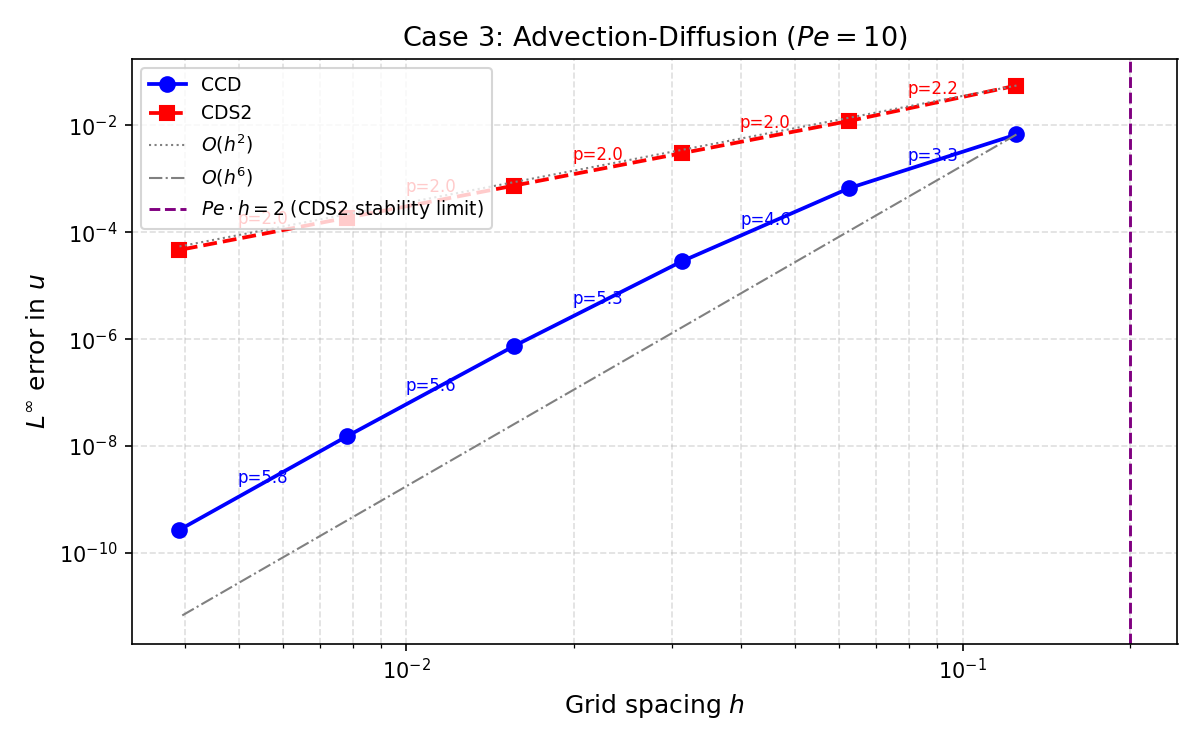
\includegraphics[width=0.72\linewidth]{figures/case3_advdiff.png}
  \caption{%
    Case 3：格子間隔 $h$ に対する $L^\infty$ 誤差の収束グラフ（両対数）．
    縦破線：$Pe \cdot h = 2$ の CDS2 安定限界（$h=0.2$）．
    CCD は漸近的に $O(h^6)$ に向かって収束次数が上昇し，
    $N=256$ で $p \approx 5.8$，CDS2 は厳密に $O(h^2)$ で収束する．
  }
  \label{fig:ccd_case3}
\end{figure}

\begin{tcolorbox}[resultbox, title={高 Péclet 境界層における CCD の優位性}]
  \begin{itemize}
    \item CCD は $N=256$（$h=1/256$）で $L^\infty = 2.71 \times 10^{-10}$ を達成し，
          同格子の CDS2（$4.68 \times 10^{-5}$）より約 17 万倍精度が高い．
    \item 収束次数は粗格子では前漸近的（$N=8$: $p=3.3$，$N=16$: $p=4.6$）だが，
          $N \geq 64$ から漸近 $O(h^6)$ に向かって安定的に上昇する（$N=256$: $p=5.8$）．
    \item CDS2 は中心差分スキームとして安定条件 $Pe \cdot h < 2$ を満たす範囲では
          $O(h^2)$ を維持するが，CCD との誤差差は格子細分化に伴い指数的に拡大する．
  \end{itemize}
\end{tcolorbox}


\subsubsection{CCD-Poisson ソルバーの単体検証（Tests C-1, C-2, C-3）}
\label{sec:ccd_poisson_verification}
\input{sections/10b_ppe_verification}
